\subsection{Componente per la struttura Phi}
\label{secphi}
L'ottenimento dell'array matching statistics permette di sapere solo
l'indice di una della righe del pannello per le quali si ha uno $\SMEM$ con
l'aplotipo query. Analogamente a quanto discusso in PHONI \cite{phoni},
anche per la $\RLPBWT$ si è pensato a due funzioni, $\varphi$ e
$\varphi^{-1}$, per il riconoscimento di tutte le
righe del pannello per le quali si ha il medesimo $\SMEM$. La componente che
permette il calcolo 
di tali funzioni è la componente denotata \texttt{PHI} e si dovrà considerare
l'assenza in memoria dei valori degli array $\RLCP$.\\
L'intuizione alla base del ragionamento è molto semplice. Nell'ordinamento alla
colonna $k$-esima, dato da $a_k$, tutte le righe, per le quali si ha un certo
$\SMEM$, sono poste consecutivamente, a causa dell'ordinamento
lessicografico inverso.
\begin{definizione}
  Dati un pannello $X$, di dimensioni $N\times M$, e una colonna $k$, avendo
  prefix array $a_k$ e permutazione inversa del prefix array $\alpha_k$, si
  definiscono formalmente: 
  \[\varphi_k(p)=
    \begin{cases}
      \NULL&\mbox{se }\alpha_k[p]=0\\
      a_k[\alpha_k[p]-1]&\mbox{altrimenti}
    \end{cases},\forall p\in\{0,M-1\}
  \]
  \[\varphi^{-1}_k(p)=
    \begin{cases}
      \NULL&\mbox{se }\alpha_k[p]=M-1\\
      a_k[\alpha_k[p]+1]&\mbox{altrimenti}
    \end{cases},\forall p\in\{0,M-1\}
  \]
  In altri termini, si ha che:
  \[\varphi_k(a_k[j])=
    \begin{cases}
     \NULL&\mbox{se }j=0\\
      a_k[j-1]&\mbox{altrimenti}
    \end{cases},\forall j\in\{0,M-1\}
  \]
  \[\varphi^{-1}_k(a_k[j])=
    \begin{cases}
      \NULL&\mbox{se }j=M-1\\
      a_k[j+1]&\mbox{altrimenti}
    \end{cases},\forall j\in\{0,M-1\}
  \]
  Quindi, dato un elemento di $a_k$, le due funzioni restituiscono il valore
  antecedente ad esso, se esistente, e il valore successivo ad esso, se
  esistente, nel prefix array. In caso di inesistenza di tale valore,
  rispettivamente ad inizio
  e fine del prefix array, si
  restituisce $\NULL$.
\end{definizione}
\dc{VERIFICARE DEFINIZIONE IN QUANTO ``NUOVA''}
\begin{esempio}
  Si ipotizzi di avere, come per l'esempio \ref{es:pbwt1}:
  \[a_6=[14,15,0,9,10,16,8,11,12,13,18,19,1,2,3,17,4,5,6,7]\]
  \[\alpha_6=[2,12,13,14,16,17,18,19,6,3,4,7,8,9,0,1,5,15,10,11]\]
  Si fissa quindi $p=3$ e si ottengono:
  \[\varphi_6(3)=a_6[\alpha_6[3]-1]=a_6[14-1]=a_6[13]=2\]
  \[\varphi^{-1}_6(3)=a_6[\alpha_6[3]+1]=a_6[14+1]=a_6[15]=17\]
\end{esempio}
Avendo, quindi, $\MS[i].\row=p$ e $\MS[i].\len=l$ basta iterare le righe a
partire da 
$p$ in $a_i$, righe che denotiamo con l'indice $q$, fino a che si ha 
$\LCE_k(x_p, x_q)\geq l$. Ovviamente bisogna iterare in entrambe le
direzioni. Tutte le righe $x_q$ che soddisfano tale condizione presentano uno
$\SMEM$ di lunghezza $l$ con 
l'aplotipo query. L'algoritmo \ref{algo:phiext} rappresenta quanto
appena descritto, avendo che la funzione $\lceb$ limita il calcolo
della 
$\LCE$ alla lunghezza desiderata $l$, escludendo computazioni inutili oltre tale
lunghezza. Tale funzione è riproducile, per mezzo di iterazioni, anche sulla
componente \texttt{RA-BV}. La complessità temporale di questo algoritmo
varia a seconda della componente per il random access (e della conseguente
presenza della 
componente \texttt{LCE}). Inoltre, è difficile poter dare una stima asintotica
in quanto varia sul numero di righe $\nu$ che presentano un certo
$\SMEM$. Quindi, si ha, con la 
componente \texttt{RA-BV}, un tempo proporzionale a:
\begin{equation}
  \label{eq:phiaccbv}
  \mathcal{O}(\nu N)
\end{equation}
Mentre con l'uso della componente \texttt{LCE}, avendo il pannello in memoria
sotto forma di $\SLP$, si ha complessità in tempo:
\begin{equation}
  \label{eq:phiaccbv2}
  \mathcal{O}(\nu\log (NM))
\end{equation}
Entrambe le stime assumono, solo per il momento, che sia possibile calcolare il
valore delle funzioni $\varphi$ e $\varphi^{-1}$ in tempo $\mathcal{O}(1)$,
avendo in 
memoria l'insieme dei prefix array (e l'insieme delle permutazioni inverse dei
prefix array) con random access in tempo costante.\\
\dc{Stime molto per eccesso, con RA-BV si scala su $l$ di fatto}
\begin{algorithm}
  \small
  \begin{algorithmic}[1]
    \Function{extend\_matches}{$k, row, len$}
    \State $haplos\gets []$
    \State $check_{down}\gets \top,\,\,check_{up}\gets \top$
    \While {$check_{down}$}
    \State $down_{row}\gets \varphi^{-1}(row, k)$
    \If{$\lceb(k, row, down_{row}, len)$}
    \State $push(haplos, down_{row})$
    \State $row \gets down_{row}$
    \Else
    \State $check_{down}\gets \bot$
    \EndIf
    \EndWhile
    \While {$up_{down}$}
    \State $up_{row}\gets \varphi(row, k)$
    \If{$\lceb(k, row, up_{row}, len)$}
    \State $push(haplos, up_{row})$
    \State $row \gets up_{row}$
    \Else
    \State $check_{up}\gets \bot$
    \EndIf
    \EndWhile
    \State \textbf{return} $haplos$
    \EndFunction
  \end{algorithmic}
  \caption{\footnotesize{Algoritmo per il calcolo di ogni $\SMEM$ in colonna $k$
  tramite la 
  componente \texttt{PHI}.}}
  \label{algo:phiext}
\end{algorithm}
\noindent
Si è presentata la definizione formale delle due funzioni ma, con la $\RLPBWT$,
si hanno in memoria solo i prefix array sample  e nessuna informazione in merito
alla permutazione inversa del 
prefix array. Non si ha in memoria nemmeno il $\RLCP$, che, in via teorica, come
per la $\BWT$, potrebbe rendere efficiente il computo delle funzioni $\varphi$
e $\varphi^{-1}$. Quindi, si è pensato ad una struttura dati, basata
anch'essa su bitvector sparsi e intvector compressi, che permettesse il calcolo
delle due funzioni senza mantenere informazioni complete in memoria. 
\subsubsection{Costruzione della struttura di supporto}
L'idea, per la costruzione della struttura a supporto delle
funzioni $\varphi$ e $\varphi^{-1}$, si
basa sul fatto che, data una colonna $k$ e dati due valori consecutivi $p$ e $q$
in $a_k$ (avendo $a_k[i]=p$ e $a_k[i+1]=q$), essi rimarranno consecutivi anche
in $a_{k+o}$ (prefix array dell'arbitraria colonna $k+o$), fino a che
che $x_{p}[k+o]\neq x_{q}[k+o]$, ovvero fino a che, in colonna $k+o$, tali righe
corrisponderanno a due simboli diversi, consecutivi nella matrice
$\PBWT$. Cruciale è che, in quella colonna, 
$p$ sarà memorizzato come prefix array sample della fine della run $r$
mentre $q$ come prefix array sample dell'inizio della run $r+1$. Grazie
a questa informazione, si può costruire una struttura che, data una colonna
arbitraria e un arbitrario valore di prefix array, permetta di
computare $\varphi$ e $\varphi^{-1}$.\\
Tale struttura dati è composta da:
\begin{itemize}
  \item un vettore di bitvector sparsi per $\varphi$, che denotiamo con
  $\varPhi$, tale che $\varPhi[i][j]=1$ sse la riga $i$ indicizza una testa di
  run alla colonna $j$, nella matrice $\PBWT$. Si ha quindi che $\varPhi$
  ha dimensione $M\times N$
  \item un vettore di bitvector sparsi per $\varphi^{-1}$, che
  denotiamo con $\varPhi^{-1}$, tale che $\varPhi[i][j]=1$ sse la riga $i$
  indicizza una coda di run alla colonna $j$, nella matrice $\PBWT$. Si ha
  quindi che $\varPhi^{-1}$ ha dimensione $M\times N$
  \item un vettore di intvector compressi, denotato $\varPhi_{supp}$, a supporto
  del vettore $\varPhi$, che memorizza, per ogni simbolo $\sigma=1$ di tale
  vettore, il 
  prefix array sample della coda della run precedente o l'altezza
  del pannello, $M$, qualora non si abbia alcuna run precedente
  \item un vettore di intvector compressi, denotato $\varPhi^{-1}_{supp}$,
  a supporto del vettore $\varPhi^{-1}$, che memorizza, per ogni simbolo
  $\sigma=1$
  di tale vettore,
  il prefix array sample della testa della run successiva o l'altezza
  del pannello, $M$, qualora non si abbia alcuna run successiva
\end{itemize}
Si ha che la lunghezza della riga $i$-esima di $\varPhi_{supp}$ è
uguale al numero di simboli $\sigma=1$ presenti nella riga $i$-esima di
$\varPhi$. Analogamente 
si ha per $\varPhi^{-1}_{supp}$. In entrambi i casi, inoltre, si hanno $M$
righe. Queste osservazioni si ripercuotono sul costo in memoria della componente
\texttt{PHI}, avendo che può essere stimata coi costi in memoria dei bitvector
sparsi e degli intvector compressi, come fatto per le precedenti componenti. Si
noti, però, che in questo caso i bitvector sparsi sono ulteriormente
ottimizzati,
avendo un rapporto davvero basso di simboli $\sigma=1$ sul totale di
simboli $N$ (e non $M$
come negli altri casi, segnalando che, in pannelli reali, $N>>M$).\\ 
Al fine della costruzione, bisogna sfruttare $a_{N-1}$ per poter
identificare quelle coppie di valori consecutivi non presenti nei vari
prefix array sample, in modo che sia possibile effettuare le query per
qualsiasi valore di prefix array in input.\\
L'algoritmo \ref{algo:phicos} riporta la costruzione della struttura,
iterando prima i vari prefix array sample e completando i
risultati con $a_{N-1}$. Tale algoritmo ha complessità in tempo, nel caso
peggiore, pari a:
\begin{equation}
  \label{eq:phicos}
  \mathcal{O}(NM)
\end{equation}
Tale caso peggiore si ha qualora ogni colonna della matrice $\PBWT$ abbia un
numero di 
run pari all'altezza stessa della colonna (un caso irrealistico). Indicando con
$\rho$ il numero medio 
di run per colonna, si ha che la complessità nel caso medio è:
\begin{equation}
  \label{eq:phicos2}
  \varTheta(N\rho)
\end{equation}
\dc{CAPIRE SE COMMENTARE ULTERIORMENTE LA COSTRUZIONE}
\begin{algorithm}
  \footnotesize
  \begin{algorithmic}[1]
    \Function{Build\_phi}{$cols, panel, prefix$}
    \Comment  $prefix=a_{N-1}$ 
    \State $\varPhi\gets [[0..0]..[0..0]],\,\,\varPhi^{-1}\gets
    [[0..0]..[0..0]]$ 
    \Comment vettori di bitvector sparsi per $\varphi$ e $\varphi^{-1}$
    \State $\varPhi_{supp} = [],\,\,\varPhi_{supp}^{-1} = []$
    \Comment vettori di intvector compressi di supporto per $\varphi$ e
    $\varphi^{-1}$  
    \For {\textit{every} $k\in [0,|cols|)$}
    \Comment costruzione da prefix array sample
    \For {\textit{every} $i\in [0,|samples_{beg}|)$}
    \State $\varPhi[sample_{beg}^{k}[i]][k]\gets 1$
    \If{$i=0$}
    \State $push(\varPhi_{supp}[sample_{beg}^{k}[i]], panel_{height})$
    \Else
    \State $push(\varPhi_{supp}[sample_{beg}^{k}[i]],sample_{end}^{k}[i-1])$
    \EndIf

    \State $\varPhi^{-1}[sample_{end}^{k}[i]][k]\gets 1$
    \If{$i=|sample_{beg}^k|-1$}
    \State $push(\varPhi_{supp}^{-1}[sample_{end}^{k}[i]], panel_{height})$
    \Else
    \State $push(\varPhi_{supp}^{-1}[sample_{end}^{k}[i]],sample_{beg}^{k}[i+1])$
    \EndIf
    \EndFor
    \EndFor
    \For {\textit{every} $k\in [0,|prefix|)$}
    \Comment costruzione da ultimo prefix array
    \If{$\varPhi[k][|\varPhi[k]|-1] = 0$}
    \State $\varPhi[k][|\varPhi[k]|-1]\gets 1$
    \If{$k=0$}
    \State $push(\varPhi_{supp}[prefix[k]], panel_{height})$
    \Else
    \State $push(\varPhi_{supp}[prefix[k]] ,prefix^k[i-1])$
    \EndIf
    \EndIf
    \If{$\varPhi^{-1}[k][|\varPhi[k]|-1] = 0$}
    \State $\varPhi^{-1}[k][|\varPhi[k]|-1]\gets 1$
    \If{$k=|prefix|-1$}
    \State $push(\varPhi^{-1}_{supp}[prefix[k]], panel_{height})$
    \Else
    \State $push(\varPhi^{-1}_{supp}[prefix[k]],prefix^k[i+1])$
    \EndIf
    \EndIf
    \EndFor
    \State \textit{costruzione della struttura $\rank$ per ogni bitvector
    sparso} 
    $\varPhi$ e $\varPhi^{-1}$
    \EndFunction
  \end{algorithmic}
  \caption{Algoritmo per la costruzione della componente \texttt{PHI}.}
  \label{algo:phicos}
\end{algorithm}
Dal punto di vista delle query, data una colonna $k$ e un valore di
prefix array $p$, per la funzione $\varphi$ si effettua  $\rank^\varphi(k)$
sulla riga $p$ di $\varPhi$, avendo che:
\[\varphi_k(p)=
  \begin{cases}
    \NULL&\mbox{se }\varPhi_{supp}^p[\rank^\varphi_p(k)]=M\\
    \varPhi_{supp}^p[\rank^\varphi_p(k)]&\mbox{altrimenti }
  \end{cases}
\]
Analogamente, per la funzione $\varphi^{-1}$ si effettua la
$rank^{\varphi^{-1}}(k)$ 
sulla riga $p$ di $\varPhi^{-1}$, avendo che:
\[\varphi_k^{-1}(p)=
  \begin{cases}
    \NULL&\mbox{se }\varPhi^{-1\,\,p}_{supp}[\rank^{\varphi^{-1}}_p(k)]=M\\
    \varPhi^{-1\,\,p}_{supp}[\rank^{\varphi^{-1}}_p(k)]&\mbox{altrimenti }
  \end{cases}
\]
In termini di complessità, si ha che tale calcolo è limitato dalla complessità
della funzione $\rank$, avendo che il numero $m$ di simboli $\sigma=1$ in ogni
bitvector, lungo $N$, equivale al numero di volte in cui la corrispondente riga
è testa/coda di una run: 
\begin{equation}
  \label{eq:queryphi}
  \mathcal{O}\left(\log\frac{N}{m}\right)
\end{equation}
\dc{Serve altro?}
\begin{esempio}
  Si supponga di avere la seguente situazione nella matrice $\PBWT$:
  \begin{figure}[H]
    \centering
    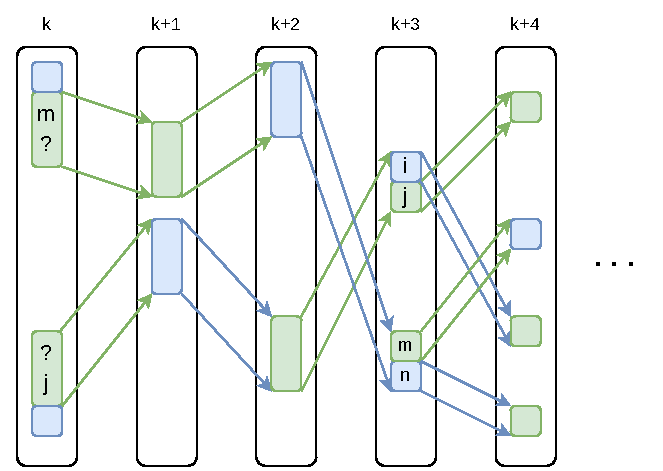
\includegraphics[scale = 0.8]{img/phi.pdf}   
  \end{figure}
  \noindent
  Dove, a parità di colore, si ha lo stesso simbolo tra due indici
  consecutivi. \\
  In colonna $k$, che per praticità assumiamo essere $k=0$, si vorrebbe avere
  informazione in merito a $\varphi_k(j)$ e $\varphi^{-1}_k(m)$. \\
  Si nota che, per definizione della struttura dati, si ha (limitandoci alle
  colonne della figura):
  \[\varPhi_j=[0,0,0,1,0, \ldots]\]
  \[\varPhi^{-1}_m=[0,0,0,1,0,\ldots]\]
  In quanto, in entrambi i casi, rispettivamente per la riga $j$ e per la riga
  $m$, 
  in colonna $k+3$, si ha che $j$ è il valore del prefix array di una testa di
  run 
  mentre $m$ di una coda di run. In colonna $k+3$ si conoscono anche,
  rispettivamente, $i$, valore del prefix array della coda della run precedente
  a quella di $j$, e $n$, valore del prefix array della testa della run
  successiva quella di $m$. Si ottengono quindi:
  \[\varPhi_{supp}=[i,\ldots]\]
  \[\varPhi^{-1}_{supp}=[n,\ldots]\]
  Si vogliono quindi calcolare $\varphi_0(j)$ e  $\varphi^{-1}_0(m)$. Si ha:
  \[\varPhi_{supp}^j[\rank^\varphi_j(0)]=\varPhi_{supp}^j[0]=i\]
  \[\varPhi^{-1\,\,m}_{supp}[\rank^{\varphi^{-1}}_m(0)]=\varPhi^{-1\,\,m}_{supp}[0]=n\]
  Si noti che uguali risultati si avrebbero per $k+1$, $k+2$ e $k+3$.
\end{esempio}
\dc{SISTEMARE UN PO' TUTTO}